%\pdfoutput=1

\documentclass[conference]{IEEEtran}
\usepackage{authblk}
\usepackage{todonotes}
\usepackage[margin=1in]{geometry}
\usepackage[parfill]{parskip}
\usepackage{times}
\usepackage{graphicx}
\usepackage{caption}
\usepackage{subcaption}
\usepackage{tikz}
\usepackage{pgfplots}
%\usepackage{natbib}
\usepackage{float}
\usepackage{algorithm,algpseudocode}
\usepackage{rotating}
%\usepackage{algorithmic}
\usepackage{amsfonts,amsmath,amsthm,amssymb}
\usepackage{mathtools}
\usepackage{hyperref}
\newcommand{\theHalgorithm}{\arabic{algorithm}}
\usepackage[shortcuts]{extdash}
\newcommand{\SREC}{S\=/REC}
\DeclareMathOperator*{\argmin}{arg\,min}
\DeclareMathOperator*{\argmax}{arg\,max}
\def\R{{\mathbb{R}}}
%\newtheorem{theorem}{Theorem}[section]
\newcommand{\mb}[1]{\mathbf{#1}}
\newtheoremstyle{exampstyle}
  {10pt} % Space above
  {10pt} % Space below
  {} % Body font
  {} % Indent amount
  {\bfseries} % Theorem head font
  {.} % Punctuation after theorem head
  {.5em} % Space after theorem head
  {} % Theorem head spec (can be left empty, meaning `normal')
\theoremstyle{exampstyle} \newtheorem{theorem}{Theorem}[section]

\newtheorem{corollary}{Corollary}[theorem]
\newtheorem{lemma}[theorem]{Lemma}
\newtheorem{definition}{Definition}
%\title{Compressed Sensing on GANs using Iterative Projections}
\title{Reconstruction from Modulo Measurements}
\date{}
\def\sgn{\mathrm{sgn}}
\def\t{\intercal}
\def\cosamp{\mathrm{CoSaMP}}
\author{Viraj Shah}
\author{Chinmay Hegde}
\affil{ECpE Department, Iowa State University}

\newcommand{\norm}[1]{\|#1\|}
\newcommand{\eps}{\epsilon}
\newcommand{\wh}[1]{\widehat{#1}}
\newcommand{\s}{0.18}
\usepackage{hyperref}
\usepackage[utf8]{inputenc}
\usepackage{booktabs}
\usetikzlibrary{calc}

\hyphenation{op-tical net-works semi-conduc-tor}
\begin{document}
\vspace{-25em}
\maketitle

%% File not in use for TSP version

%\section{Mathematical Model}
%\label{sec:mathmod}
%We consider the problem of recovery of a signal from its modulo measurements obtained through compressive sensing. Simply put, we aim to recover $\mathbf{x^*}\in \R^n$ from the modulo measurements $y_i$ defined as:
%
%\begin{equation}
%y_i=\mod(\langle \mathbf{a_i} \cdot \mathbf{x^*} \rangle,R)~\textnormal{for}~i = \{1,2,...,m\},
%\end{equation} 
%
%
%where $\mod(\cdot)$ is modulo operation with respect to a fixed, real-valued parameter $R$. Typically, $m<n$. For simplicity, we assume that the modulo function operates only within two periods, one each on the either side of the origin, as shown in the Fig.~\ref{fig:graph}. We construct $\mathbf{A} = \left[\mathbf{a_1~a_2~...~a_m}\right]^T$ with i.i.d. Gaussian entries. The primary assumption in our model is that the natural signal $\mathbf{x^*}$ is $s-$sparse in a chosen basis. 
%
%\begin{figure}[h]
%	\begin{center}
%\begin{tikzpicture}[scale=0.7, every node/.style={scale=0.7}]
%\draw[<->] (-4,0) -- (4,0) node[right] {$t$};
%\draw[->] (0,-1) -- (0,4) node[above] {$f(t)$};
%\draw[scale=0.5, dashed, thick] (0,4)--(7,4) node[right]{$R$};
%\draw (1.5,-0.5) node(below) {$p_i = 0$};
%\draw (-1.5,-0.5) node(below) {$p_i = 1$};
%\draw (0,-1.5) node(right) {$f(t) = \mod(t,R)$};
%\draw[scale=0.5,domain=-7:0,smooth,variable=\x,cyan, ultra thick] plot ({\x},{\x+4});
%\draw[scale=0.5,domain=0:7,smooth,variable=\x,cyan, ultra thick]  plot ({\x},{\x});
%\end{tikzpicture}
%\end{center}
%\caption{\emph{Modified modulo function chosen in our problem}}
%\label{fig:graph}
%\end{figure}
%
%We can write the modified equation for the modulo operation under consideration as:
%$$
%f(t) = \mod(t,R) = t+\left( \frac{1-\sgn(t)}{2}\right)R,
%$$
%where $\sgn(t)$ is a signum function.
%
%For the measurement model of the given problem, 
%We define the corrected linear measurements as: 
%
%$$
%y_{c,i} =\langle \mathbf{a_i} \cdot \mathbf{x^*} \rangle.
%$$
%
%We also define each element of the true bin-index vector $\mb{p^*}$ as,
%$$
%p^*_i = \frac{1-\sgn(\langle \mathbf{a_i} \cdot \mathbf{x^*} \rangle)}{2}.
%$$
%Thus,
%$$
%y_i = \langle \mathbf{a_i} \cdot \mathbf{x^*} \rangle + p^*_iR = y_{c,i}+p^*_iR.
%$$
%
%It is evident that if we can recover $\mathbf{p^*}$ successfully, we can calculate the correct compressed measurements $\langle \mathbf{a_i} \cdot \mathbf{x^*} \rangle$ and use them to reconstruct $\mathbf{x^*}$ with any sparse recovery algorithm such as CoSaMP.
%
%
%\section{Reconstruction Algorithm}
%
%In this section, we describe our AltMin based approach to recover $\mathbf{x^*}$ and $\mathbf{p^*}$, given $\mathbf{y, A}, s, R$. We call our algorithm MoRAM - Modulo Reconstruction using Alternative Minimization. Our approach comprises of two steps: (i) initialization step, and (ii) Descent step through alternative minimization.
%
%\subsection{Initialization using Re-Calculated Measurements (RCM)}
%\label{sec:init}
%Similar to other non-convex approaches, MoRAM also requires an initial estimate $\mathbf{{x}^0}$ that is close to the true signal $\mathbf{{x}^*}$. We have several initialization techniques available, typically used in phase retrieval problems; such as spectral initialization. However, the nature of the problem in our case is fundamentally different due to asymmetric and non-linear behavior of the modulo transfer function. To overcome this issue, we propose a method to re-calculate the true measurements ($\mb{y_c}= \mb{Ax^*}$) from the available modulo measurements. We aim to undo the effect of modulo operation for the fraction of the total measurements. To understand the method for such re-calculation, we will first try to understand the effect of modulo operation on the linear measurements.
%
%\subsubsection{The effect of modulo operation} 
%\label{sec:modeff}
%We observe the density distributions of the $\mathbf{Ax^*}$(Fig.~\ref{fig:hist1}) and $\mathbf{\mod(\mathbf{Ax^*})}$(Fig.~\ref{fig:hist2}) to understand the information we can obtain from the modulo measurements. We are particularly interested in the case where signal strengths are low compared to the value of $R$, nevertheless, we also analyze the other case when $R$ is less than the signal strength. Here, we approximate the spread of the $\mathbf{Ax^*}$ with a hyper-parameter $\rho$. We choose a value of $\rho$ such that it bounds the maximum element of $|\mathbf{Ax^*}|$ with very high probability.
%In Fig.~\ref{fig:hist2} and Fig.~\ref{fig:hist3}, we can see the histogram after modulo operation for both the cases: $R>\rho$ and $R<\rho$. Comparing these histograms with the histogram of true measurements (Fig.~\ref{fig:hist1}), we can observe how the values of first histogram translates into second or third when the modulo operation is applied. We can draw following conclusions:
%\begin{itemize}
%	\item Only the values lying on the negative side of the x-axis are going to be affected.
%	\item Values lying very close to the origin on the negative side of the x-axis in the first histogram, would now shift by $R$, and would occupy a place very close to $R$ in second histogram. For $R>\rho$, this region is shaded with green color in Fig.~\ref{fig:hist2}. Correct bin-value for the elements in $\mathbf{y}$ with value lying between $\rho$ and $R$ is $p_{rcm,i} = 1$.
%	\item For $R>\rho$, histogram of the positive region very close to the origin would remain unaffected. This region is shaded with orange color in Fig.~\ref{fig:hist2}. Correct bin-value for all the elements in $\mathbf{y}$ with value lying between $0$ and $R-\rho$ is $p_{rcm,i} = 0$.
%	\item Nothing can be concluded for measurements lying in between the above mentioned ranges. This region is shaded with gray color in Fig.~\ref{fig:hist2} and Fig.~\ref{fig:hist3}. Correct bin-value cannot be identified for this region, so we assign all the elements in $\mathbf{y}$ with value lying between $0$ and $(R-\rho)$ as $p_{rcm,i} = 0$. The lower and upper bounds ($t_l \& t_u$) of this disputed region can be obtained as, 
%	$$t_l = \max(0, R-\rho)$$
%	$$t_u = \max(\rho, R)$$.
%	\item Irrespective of relationship between $\rho$ and $R$, all the values lying in the negative half of the real line have the bin-value equal to $1$, and all the values greater than $R$ have the bin-value equal to $0$.
%\end{itemize}
%
%\begin{algorithm}[t]
%	\caption{\textsc{RCM-Initialization}}
%	\label{alg:RCM}
%	\begin{algorithmic}
%		\State\textbf{Inputs:} $\mathbf{y}$, $\mathbf{A}$, $s$, $R$, $\rho$
%		\State\textbf{Output:}  $\mb{x^0}$
%		\State $T \leftarrow \phi$, $t_l \leftarrow \max(0, R-\rho)$, $t_u \leftarrow \max(\rho, R)$
%		\For {$l= 0:m$}
%		\If {$y_l<0$}
%		\State {$p^{rcm}_l = 1$, $T \leftarrow T \cup {l}$}
%		\ElsIf {$0\leq y_l < t_l$}
%		\State {$p^{rcm}_l = 0$, $T \leftarrow T \cup {l}$}
%		\ElsIf {$t_l\leq y_l < t_u$}
%		\State {$p^{rcm}_l = 0$}
%		\ElsIf {$t_u \leq y_l < R$}
%		\State {$p^{rcm}_l = 1$, $T \leftarrow T \cup {l}$}
%		\ElsIf {$R  \leq y_l$}
%		\State {$p^{rcm}_l = 0$, $T \leftarrow T \cup {l}$}
%		
%		\EndIf	
%		\EndFor
%		\State $N \leftarrow |T|$
%		\State $\mb{x^0} \leftarrow H_s\left( \frac{1}{N}\sum_{i=1}^{N}y_{T,i}a_{T,i}\right)$
%	\end{algorithmic}
%\end{algorithm}
%
%
%
%
%\begin{figure}[h]
%	\begin{center}
%		\begin{tikzpicture}[scale=0.7, every node/.style={scale=0.7}]
%		\def\normaltwo{\x,{3*1/exp(((\x)^2)/2)}}
%		\def\y{4.4}
%		
%		\fill [fill=orange!60] (2.6,0) -- plot[domain=0:4.4] (\normaltwo) -- ({\y},0) -- cycle;
%		
%		 Draw and label normal distribution function
%		\draw[color=blue,domain=-3:3,thick] plot (\normaltwo) node[right] {};
%		\draw[<->] (-5,0) -- (5,0) node[right] {$\mathbf{Ax^*}$};
%		\draw[<->] (0,-1) -- (0,4);
%		
%		\draw (-3,-0.5) node(below) {$-\rho$};
%		\draw (-4,-0.5) node(below) {$-R$};
%		\draw (3,-0.5) node(below) {$\rho$};
%		\draw (4,-0.5) node(below) {$R$};
%		
%		\foreach \x in {-3,-4,3,4}
%		{        
%			\coordinate (A\x) at ($(0,0)+(\x*1cm,0)$) {};
%			\draw ($(A\x)+(0,5pt)$) -- ($(A\x)-(0,5pt)$);
%			
%		}
%				\draw (-1.5,-0.5) node(below) {$p_i = 1$};
%				\draw (0,-1.5) node(right) {$f(t) = \mod(t,R)$};
%				\draw[scale=0.5,domain=-7:0,smooth,variable=\x,cyan, ultra thick] plot ({\x},{\x+4});
%				\draw[scale=0.5,domain=0:7,smooth,variable=\x,cyan, ultra thick]  plot ({\x},{\x});
%		\end{tikzpicture}
%	\end{center}
%	\caption{\emph{Histogram of $\mathbf{Ax^*}$}}
%	\label{fig:hist1}
%\end{figure}
%\begin{figure}[h]
%	\begin{center}
%		\begin{tikzpicture}[scale=0.7, every node/.style={scale=0.7}]
%		\def\normaltwo{\x,{3*1/exp(((\x)^2)/2)}}
%		\def\normalone{\x,{3*1/exp(((\x-4)^2)/2)}}
%		\def\normalsum{\x,{3*1/exp(((\x-4)^2)/2)+3*1/exp(((\x)^2)/2)}}
%		\def\y{3}
%		\def\fy{3*1/exp(((\y-4)^2)/2)}
%		\fill [fill=orange!60] (0,0) -- plot[domain=0:1] (\normaltwo) -- (1,0) -- cycle;
%		\fill [fill=green!60] (3,0) -- plot[domain=3:4] (\normalone) -- (4,0) -- cycle;
%		\fill [fill=gray!30] (1,0) -- plot[domain=1:3] (\normalsum) -- (3,0) -- cycle;
%		 Draw and label normal distribution function
%		\draw[color=blue,domain=-0:3,dashed,thick] plot (\normaltwo) node[right] {};
%		\draw[color=blue,domain=1:4,dashed,thick] plot (\normalone) node[right] {};
%		\draw[color=blue,domain=-0:4,thick] plot (\normalsum) node[right] {};
%		\draw[<->] (-5,0) -- (5,0) node[right] {$\mathbf{Ax^*}$};
%		\draw[<->] (0,-1) -- (0,4);
%		\draw[dashed] ({\y},{\fy}) -- ({\y},0);
%		\draw[dashed] ({4},{3}) -- ({4},0);
%		\draw[dashed] ({1},{\fy}) -- ({1},0);
%		\draw (-3,-0.5) node(below) {$-\rho$};
%		\draw (-4,-0.5) node(below) {$-R$};
%		\draw (3,-0.5) node(below) {$\rho$};
%		\draw (4,-0.5) node(below) {$R$};
%		\draw (1,-0.5) node(below) {$R-\rho$};
%		\draw (0.5,1) node(below) {$p_i=0$};
%		\draw (3.5,1) node(below) {$p_i=1$};
%		\draw (2,0.5) node(below) {$p_i=0$};
%		\foreach \x in {-3,-4,1,3,4}
%		{        
%			\coordinate (A\x) at ($(0,0)+(\x*1cm,0)$) {};
%			\draw ($(A\x)+(0,5pt)$) -- ($(A\x)-(0,5pt)$);
%			
%		}
%				\draw (-1.5,-0.5) node(below) {$p_i = 1$};
%				\draw (0,-1.5) node(right) {$f(t) = \mod(t,R)$};
%				\draw[scale=0.5,domain=-7:0,smooth,variable=\x,cyan, ultra thick] plot ({\x},{\x+4});
%				\draw[scale=0.5,domain=0:7,smooth,variable=\x,cyan, ultra thick]  plot ({\x},{\x});
%		\end{tikzpicture}
%	\end{center}
%	\caption{\emph{Histogram of $\mod(\mathbf{Ax^*})$, $R>\rho$}}
%	\label{fig:hist2}
%\end{figure}
%
%\begin{figure}[!h]
%	\begin{center}
%		\begin{tikzpicture}[scale=0.7, every node/.style={scale=0.7}]
%		\def\normaltwo{\x,{3*1/exp(((\x)^2)/2)}}
%		\def\normalone{\x,{3*1/exp(((\x-2)^2)/2)}}
%		\def\normalsum{\x,{3*1/exp(((\x-2)^2)/2)+3*1/exp(((\x)^2)/2)}}
%		\def\y{3}
%		\def\fy{3*1/exp(((\y-4)^2)/2)}
%		\fill [fill=orange!60] (-1,0) -- plot[domain=-1:0] (\normalone) -- (0,0) -- cycle;
%		\fill [fill=green!60] (2,0) -- plot[domain=2:3] (\normaltwo) -- (3,0) -- cycle;
%		\fill [fill=gray!30] (0,0) -- plot[domain=0:2] (\normalsum) -- (2,0) -- cycle;
%		 Draw and label normal distribution function
%		\draw[color=blue,domain=-0:3,dashed,thick] plot (\normaltwo) node[right] {};
%		\draw[color=blue,domain=-1:2,dashed,thick] plot (\normalone) node[right] {};
%		\draw[color=blue,domain=-0:2,thick] plot (\normalsum) node[right] {};
%		\draw[<->] (-5,0) -- (5,0) node[right] {$\mathbf{Ax^*}$};
%		\draw[<->] (0,-1) -- (0,4);
%		\draw[dashed] ({\y},{\fy}) -- ({\y},0);
%		\draw[dashed] ({-1},{2}) -- ({-1},0);
%		\draw[dashed] ({3},{2}) -- ({3},0);
%		\draw[dashed] ({1},{\fy}) -- ({1},0);
%		\draw (-3,-0.5) node(below) {$-\rho$};
%		\draw (-2,-0.5) node(below) {$-R$};
%		\draw (3,-0.5) node(below) {$\rho$};
%		\draw (2,-0.5) node(below) {$R$};
%		\draw (-1,-0.5) node(below) {$-\rho+R$};
%		\draw (-0.5,1) node(below) {$p_i=0$};
%		\draw (2.5,1) node(below) {$p_i=1$};
%		\draw (1,0.5) node(below) {$p_i=0$};
%		\foreach \x in {-3,-2,-1,3,2}
%		{        
%			\coordinate (A\x) at ($(0,0)+(\x*1cm,0)$) {};
%			\draw ($(A\x)+(0,5pt)$) -- ($(A\x)-(0,5pt)$);
%			
%		}
%				\draw (-1.5,-0.5) node(below) {$p_i = 1$};
%				\draw (0,-1.5) node(right) {$f(t) = \mod(t,R)$};
%				\draw[scale=0.5,domain=-7:0,smooth,variable=\x,cyan, ultra thick] plot ({\x},{\x+4});
%				\draw[scale=0.5,domain=0:7,smooth,variable=\x,cyan, ultra thick]  plot ({\x},{\x});
%		\end{tikzpicture}
%	\end{center}
%	\caption{\emph{Histogram of $\mod(\mathbf{Ax^*})$, $R<\rho$}}
%	\label{fig:hist3}
%\end{figure}
%We divide the number line in the following 5 intervals, and assign the bin-value accordingly:
%\begin{equation}
%{p}^{rcm}_{i} = 
%\begin{cases}
%1,& \text{if } y_i <0 \\
%0,& \text{if } 0\leq y_i < t_l \\
%0,& \text{if } t_l\leq y_i < t_u ~~~~ \textnormal{(region of uncertainity)} \\
%1,& \text{if } t_u \leq y_i < R \\
%0,& \text{if } R  \leq y_i. \\
%\end{cases}
%\label{eq:rcm}
%\end{equation}
%Thus, we can identify the correct bin values for part of the measurements just by observing their magnitude. We define set $T$ as the set of measurements for which we can identify the bin-values correctly. We introduce $N=:|T|$.
%\begin{align*}
%N & =  m - \textnormal{number of measurements lying} \\
%     &~~~\textnormal{in the region of uncertainity}
%\end{align*}
%Value of $N$ largely depends on the difference between $\rho$ and $R$.
%
%Once we identify the correct bin-values for part of the measurements, we can re-calculate corrected measurements as,
%$$
%\mathbf{y_{c} = y + p^{rcm}R}.
%$$
%We use these corrected measurements $\mathbf{y_{rcm}}$ to calculate the initial estimate $\mathbf{{x}^0}$ using the estimation step described in the upcoming section.
%\subsubsection{Calculating the initial estimate from the corrected measurements}
%In the estimation step, $\mb{x^0}$ is calculated only from the $N$ corrected measurements using first order unbiased estimator. For that, we use the versions of $\mb{y}$ and $A$ truncated to the indices belong to set $T$:
%\begin{equation}
%\mb{x^0} = H_s\left( \frac{1}{N}\sum_{i=1}^{N}y_{T,i}a_{T,i}\right)
%\label{eq:init}
%\end{equation}
%where $H_s$ denotes the hard thresholding operator that keeps the $s$ largest absolute entries of a vector and sets the other entries to zero.
%\subsection{Alternative Minimization}
%\label{sec:altmin}
%\begin{algorithm}[H]
%	\caption{\textsc{MoRAM}}
%	\label{alg:MoRAM}
%	\begin{algorithmic}
%		\State\textbf{Inputs:} $\mathbf{y}$, $\mathbf{A}$, $s$, $R$
%		\State\textbf{Output:}  $\widehat{x}$
%		\State $m,n \leftarrow \mathrm{size}(\mathbf{A})$ 
%		\State \textbf{Initialization}
%		\State $\mathbf{x^0} \leftarrow \textrm{RCM}(\mathbf{y, A})$ 
%		\State \textbf{Alternative Minimization}
%		\For {$l =0:\mathrm{maxiter}$}
%		\State $\mathbf{{p}^{t}} \leftarrow \frac{\mathbf{1}-\sgn(\langle \mathbf{A} \cdot \mathbf{x^t} \rangle)}{2}$
%		\State $\mathbf{y^t_c} \leftarrow \mathbf{y} - \mathbf{p^t}R$
%		\State $\mathbf{{x}^{t+1}}\leftarrow \argmin_{\mb{u}=[\mathbf{x~d}]^T}\norm{u}_1  s.t.~ \begin{bmatrix} \mathbf{A} & \mathbf{I} \end{bmatrix}\mb{u} = \mathbf{y}$ 
%		\State $\implies \mathbf{{x}^{t+1}}\leftarrow \small{JP(\frac{1}{\sqrt{m}}\begin{bmatrix} \mathbf{A} & \mathbf{I} \end{bmatrix},\frac{1}{\sqrt{m}}\mathbf{y},[\mathbf{x^t~~p^t}]^T)}$.
%		\EndFor
%	\end{algorithmic}
%\end{algorithm}
%
%
%Using Eq.~\ref{eq:init}, we calculate the initial estimate of the signal $\mathbf{{x}^0}$ which is relatively close to the true vector $\mathbf{x^*}$. Starting with $\mathbf{{x}^0}$, we  calculate the estimates $\mathbf{p}$ and $\mathbf{x}$ in alternating fashion to converge to the original signal $\mathbf{x^*}$. At each iteration of our Alternative Minimization, we use the current estimate of the signal ${\mathbf{x^t}}$ to get the value of the bin-index vector $\mathbf{{p}^t}$ as following:
%\begin{equation}
%\mathbf{{p}^{t}} = \frac{\mathbf{1}-\sgn(\langle \mathbf{A} \cdot \mathbf{x^t} \rangle)}{2}.
%\label{step1}
%\end{equation}
%
% 
% Given $\mathbf{x^0}$ is close to $\mathbf{x^*}$, $\mathbf{p^0}$ would also be close to $\mathbf{p^*}$. Ideal way is to calculate the correct compressed measurements $\mathbf{y^t_c}$ using $\mathbf{p^t}$, and use $\mathbf{y_c}$ with CoSaMP to calculate the next estimate $\mathbf{{x}_{t+1}}$. Thus,
%
%
%$$
%\mathbf{y^t_c} = \langle \mathbf{A}\mathbf{x^{t}} \rangle = \mathbf{y} - \mathbf{p^t}R,
%$$
%$$
%\mathbf{{x}^{t+1}} = \argmin_{\mathbf{x} \in \mathcal{M}_s}\norm{\mathbf{Ax} - \mathbf{y^t_c}}_2^2, %~~\mathrm{s.to}~~x^* \in \mathcal{M}_s,
%$$
%
%\begin{equation}
%\implies \mathbf{{x}^{t+1}} = \cosamp(\frac{1}{\sqrt{m}}\mathbf{A},\frac{1}{\sqrt{m}}\mathbf{y^t_c},s,\mathbf{x^t}).
%\label{eq:cosamp}
%\end{equation}
%
%
% However, it should be noted that even the small error $\mathbf{d} = \mathbf{p^t - p^*}$ would reflect heavily in the calculation of $\mathbf{y^t_c}$, as each incorrect bin-index would add a noise of the magnitude $R$ in $\mathbf{y^t_c}$. Experiments suggest that the CoSaMP is not robust enough to cope up with such large errors in $\mathbf{y^t_c}$. To tackle this issue, we augmented the sparse recovery problem using the fact that the nature of error $\mathbf{d^t_p}$ is sparse; and each erroneous element of $\mathbf{p}$ adds a noise of the magnitude $R$ in $\mathbf{y^t_c}$. We take the sparsity of $\mathbf{d^t}$ to be $s_p = 0.1\times m$, suggesting that at most the $10\%$ of the total elements are classified with wrong bin-indices.
% 
% The augmented optimization problem becomes,
%  
%$$
%\mathbf{{x}^{t+1}}=\argmin_{[\mathbf{x~d}]^T \in \mathcal{M}_{s+s_p}}\norm{\begin{bmatrix} \mathbf{A} & \mathbf{I} \end{bmatrix} \begin{bmatrix} \mathbf{x} \\ \mathbf{d} \end{bmatrix} - \mathbf{y^t_c}}_2^2, %~~\mathrm{s.to}~~x^* \in \mathcal{M}_s,
%$$
%\begin{equation}
%= \cosamp(\frac{1}{\sqrt{m}}\begin{bmatrix} \mathbf{A} & \mathbf{I} \end{bmatrix},\frac{1}{\sqrt{m}}\mathbf{y_c^t},s+s_p,[\mathbf{x^t~~p^t}]^T).
%\label{eq:robcosamp}
%\end{equation}
%We call the step in Eq.~\ref{eq:robcosamp} a Robust CoSaMP. 
%However, for using CoSaMP , it is required to specify the total sparsity value $(s +s_p)$, where $s_p$ is unknown. Thus, we employ Basis pursuit instead of CoSaMP, which doesn't rely on sparsity. The robust formulation of basis pursuit is referred as Justice Pursuit (JP) in the literature, specified in Eq.~\ref{eq:jp}.
%\begin{equation}
%\implies \mathbf{{x^{t+1}}} = JP(\frac{1}{\sqrt{m}}\begin{bmatrix} \mathbf{A} & \mathbf{I} \end{bmatrix},\frac{1}{\sqrt{m}}\mathbf{y^t_c},[\mathbf{x^t~~p^t}]^T).
%\label{eq:jp}
%\end{equation}
%We repeat the steps of bin index calculation (as in Eq.~\ref{step1}) and sparse recovery (as in Eq.~\ref{eq:cosamp} or Eq.~\ref{eq:robcosamp} or Eq.~\ref{eq:jp}) alternatively for $\mathrm{N}$ iterations. While the sparse recovery with robust CoSaMP (Eq.~\ref{eq:robcosamp}) improves the reconstruction performance for large values of $R$ by making the sparse recovery step less susceptible to the errors, CoSaMP can also used in its original form (as in Eq.~\ref{eq:cosamp}) for lower values of $R$. Nevertheless, the best performing recovery algorithm uses Justice Pursuit, which is able to produce perfectly converging results, as described in experimental section.
%
%Thus, we can have two variants of the MoRAM algorithm: (i)MoRAM with CoSaMP, (ii) MoRAM with robust CoSaMP, and (iii) MoRAM with Justice Pursuit. 
%
%$$
%\norm{\begin{bmatrix} \mathbf{A} & \mathbf{I} \end{bmatrix} \begin{bmatrix} \mathbf{x^*} \\ \mathbf{d} \end{bmatrix} - \mathbf{y}}_2^2.
%$$
%
%

\newpage

\section{Mathematical Analysis}

\subsection{Analysis of the Initialization}
We perform the initialization in two steps:
(i) Measurement correction step, (ii) Estimation step.

\subsubsection{Measurement correction step}: In this step, based on the absolute value of the modulo measurements, we identify the measurements for which we can undo the effect of the modulo operation by guessing the correct value of $\mathbf{p}$. We define the set $T$ as set of indices of all such measurements.

We determine the measurements to be corrected based on the method described in section~{\todo{add section}}. 
In this analysis, our goal is to find out the total number of measurements ($N=|T|$), that can be corrected through the \todo{histogram analysis -  change the term}. Only these $N$ measurements would be used in the estimation step.
Each element of $A$ id i.i.d. standard normal, thus, $\mu_{A_{ij}} = 0$ and $\sigma_{A_{ij}}=1$.
$$
y_{c,i} =\langle \mathbf{a_i} \cdot \mathbf{x^*} \rangle = \sum_{j=1}^{n}A_{ij}x^*_{j}.
$$

So, 
$$
y_{c,i} \sim \mathcal{N}\left(\mu= \sum_{j=1}^{n}x^{*}\mu_{A_{ij}}, \sigma =\sum_{j=1}^{n}x^{*2}_{j}\sigma^2_{A_{ij}}\right)
$$
$$
\implies y_{c,i} \sim \mathcal{N}\left(\mu= 0, \sigma =\sum_{j=1}^{n}x^{*2}_{j} = \norm{\mathbf{{x}^*}}^2 = 1 \right)
$$

Here, each element of $\mathbf{y_c}$ follows a zero mean Gaussian distribution with unit variance.

Now to calculate $N$, we consider the following result:
We can calculate $N$ using the fact that the measurements follow the standard normal distribution, and the total number of measurements are $m$.
Number of measurements lying in the interval $[\alpha,\beta]$ = $mP(\alpha \leq y_{c,i}\geq \beta) = m\left(Q(\alpha)- Q(\beta)\right)$; \\
Where, $Q(\cdot)$ is Q-function, defined as, $Q(t) = 1-\Phi(t)$ with $\Phi(\cdot)$ being CDF of standard normal distribution. \\
We also note that $Q(-t) = 1 - Q(t)$. \\
Q-function is not an elementary function. However, it can be bounded by following functions where $\phi(\cdot)$ is standard normal density function:
$$
\left(\frac{t}{1+t^2}\right)\phi(t) < Q(t) < \frac{\phi(t)}{t}.
$$

case (i) $R > \rho$: in this case, \\
$N$ = number of measurements lying in the interval $[-R + \rho,0]$ + number of measurements lying in the interval $[0, R-\rho]$.
\begin{equation}
N = m\left(Q(-R+\rho)- Q(0)\right) + m\left(Q(0)- Q(R-\rho)\right)
~~ = m\left(Q(-(R-\rho))- Q(R-\rho)\right) 
~~ = m\left(1-2Q(R-\rho)\right)
\end{equation}

Using the above bounds,
$$
N \geq m \left(1-2\frac{\phi(R-\rho)}{(R-\rho)} \right)
$$

case (ii) $R < \rho$: in this case, \\
$N$ = number of measurements lying in the interval $[-\rho,-R]$ + number of measurements lying in the interval $[R,\rho]$.
\begin{equation}
N = m\left(Q(-\rho)- Q(-R)\right) + m\left(Q(R)- Q(\rho)\right)
~~ = m\left(1 - Q(\rho)-1 +Q(R) +Q(R) -Q(\rho)\right) 
~~ = 2m\left(Q(R)-Q(\rho)\right)
\end{equation}

Using the above bounds,
$$
N \geq 2m \left(\frac{R}{(1+R^2)} \phi(R) - \frac{\phi(\rho)}{\rho}\right)
$$


\subsubsection{Estimation step}

We calculate the initial estimate using the measurements in set $T$ as following,
$$
\mathbf{{x}^0} = M = \frac{1}{|T|}\sum_{i\in T}y_{i}a_{i}.
$$

We use the versions of $\mb{y}$ and $A$ truncated to the indices belong to set $T$.
$$
\mathbf{{x}^0} = M = \frac{1}{N}\sum_{i=1}^{N}y_{T,i}a_{T,i} =  \frac{1}{N}A^T\mb{y_T}.
$$
Substituing $\mb{y_T}=A_T\mb{x^*}$,
$$
\mathbf{{x}^0} = M = \frac{1}{N}A_T^\t A_T\mb{x^*}.
$$

We note that each row of our Gaussian measurement matrix ($A_{T,i}$) is independent, and also follows the Guassian distribution with zero mean.  
We denote this distribution with Gaussian random vector $Z$ in $\R^n$, and arrange $N$ rows as the independent samples from the distribution; $Z_i := A_{T,i}$. 

Recall that the covariance matrix of $Z$ can be calculated as $\Sigma = \mathbb{E}Z\otimes Z$,
$$
\Sigma= \mathbb{E}Z\otimes Z = \mathbb{E} ZZ^\t = diag(\mathbb{E}z_1^2,\mathbb{E}z_2^2,...,\mathbb{E}z_n^2) = I_n
$$

Now, calculating the sample covariance matrix of $Z$ using the samples $Z_i = A_{T,i}$,
$$
\Sigma_N = \frac{1}{N}\sum_{i=1}^{N}Z_i \otimes Z_i = \frac{1}{N} A_T^\t A_T
$$
Let $\epsilon \in (0,1), t\geq 1$,
We invoke the Corrolary 5.50 of \cite{} \todo{cite vershynin},
\theorem{Let $\epsilon\in (0,1)$ and $t \geq 1$. The initial estimate $\mb{x^0}$ is the output of the algorithm \todo{add algo ref}. If the total number of corrected measurements satisfy, $N \geq C(\frac{t}{\epsilon})^2n$, then  with probability at least $1 - 2\exp\left(-t^2n\right)$ we have,
$$
\norm{\mb{x^0} - \mb{x^*}}_2 \leq \epsilon \norm{\mb{x^*}}_2.
$$
}

\begin{align*}
\norm{\Sigma_N - \Sigma} &\leq \epsilon \\
\implies \norm{\frac{1}{N} A_T^\t A_T - I_n} &\leq \epsilon \\
\implies \sup_{\mb{x} \in \R^n} \frac{\norm{\left(\frac{1}{N} A_T^\t A_T - I_n\right)\mb{x}}_2}{\norm{\mb{x}}_2} &\leq \epsilon \\
\implies \norm{\left(\frac{1}{N} A_T^\t A_T - I_n\right)\mb{x^*}}_2 &\leq \epsilon \norm{\mb{x^*}_2} \\
\implies \norm{\left(\frac{1}{N} A_T^\t A_T\mb{x^*} - \mb{x^*}\right)}_2 &\leq \epsilon \norm{\mb{x^*}_2} \\
\implies \norm{\mb{x^0} - \mb{x^*}}_2 &\leq \epsilon \norm{\mb{x^*}}_2 \\
\end{align*}


\subsection{Analysis of the Convergence}
We perform the Alternative Minimization Algorithm as described in~\ref{alg:MoRAM}, starting with $\mb{x^0}$ calculated as above. 
The first step is to obtain the initial estimate for bin-index vector, $\mb{p^0}$ using $\mb{x^0}$.
$$
\mathbf{{p}^{0}} = \frac{\mathbf{1}-\sgn(\langle \mathbf{A} \cdot \mathbf{x^0} \rangle)}{2}.
$$
If we try to undo the effect of modulo operation by adding back $R$ for the affected measurements based on the bin-index vector $\mb{p^0}$, it would introduce the error equaling $R$ corresponding to the incorrect bin-index values in $\mb{p^0}$.
$$
\mathbf{y^0_c} = \langle \mathbf{A}\mathbf{x^{0}} \rangle = \mathbf{y} - \mathbf{p^0}R,
$$

If the initial bin-index vector $\mb{p^0}$ is close to the true bin-index vector $\mb{p^*}$, then the fraction of noisy measurements in $\mb{y^0_c}$ with respect to total number of measurements $m$ is small enough to treat $\mb{y^0_c}$ as sparsely corrupted measurements. Unlike the general cases of noise, in this case the corruption cannot be modeled as a probability distribution. However, if we model this corruption as a sparse noise, then we can employ Justice Pursuit for a guaranteed recovery of the true signal given (i) sparsity of the noise is a fraction of total number of measurements; (ii) sufficiently large number of measurements are available. In the following theorem, we claim the guaranteed recovery of the true signal as the corruption in the first set of corrected measurements $\mb{y_c^0}$ can be modeled as sparse vector with sparsity less than or equal to $Cm$, with $C$ being a fraction. 

\lemma{Let $\mb{A}$ be the matrix generated as $\mb{A} \sim \mathcal{N}^{m \times n}(0,1)$ and $\mb{x^*, x^0} \in \R^n$ are $s-$sparse vectors satisfying $\norm{\mb{x^* - x^0}}_2 \leq \delta_1$. Let $\epsilon \in (0,1)$. Given the number of measurements $m \geq ***$, following is true with probability exceeding $1 - (****)$:
	
	$$
	d_H(\sgn({\mb{Ax^*}}), \sgn({\mb{Ax^0}})) \leq \delta_1 + \epsilon;
	$$
where $d_H$ is Hamming distance between binary vectors defined as:

$$
d_H(\mb{a,b}) =: \frac{1}{n}\sum_{i=1}^{n}a_i \oplus b_i \textnormal{~~for $n-$ dimensional binary vectors~} \mb{a,b}.
$$ 
}
\textit{Proof.} For proof, we first introduce the concept of binary $\epsilon$-stable embedding as appears in \todo{cite jacques}.
\definition[Binary $\epsilon$-Stable Embedding]{A mapping $F: \R^n \rightarrow \mathcal{B}^m$ is a binary $\epsilon$-stable embedding (B$\epsilon$SE) of order $s$ for sparse vectors if:
$$
d_S(\mb{x,y}) - \epsilon \leq d_H(F\mb{(x)},F\mb{(y)}) \leq d_S(\mb{x,y}) + \epsilon;
$$
for all $\mb{x,y} \in S^{n-1}$ with $|supp(x) \cup supp(y)|\leq s$.
}
 
In our case, let's define the mapping $F: \R^n \rightarrow \mathcal{B}^m$ \todo{add definition of Bm} as:
$$
F(\mb{x})=: \sgn(\mb{Ax});
$$
with $\mb{A} \sim \mathcal{N}^{m \times n}(0,1)$.

Given $m > ****$, using Theorem 3 from \todo{cite jacques} we conclude that $F$ is a B$\epsilon$SE for $s$-sparse vectors.
Thus for sparse vectors $\mb{x^*, x^0}$:
$$
d_H(F\mb{(x^*)},F\mb{(x^0)}) \leq d_S(\mb{x^*,x^0}) + \epsilon
$$

$$
\implies d_H(\sgn({\mb{Ax^*}}), \sgn({\mb{Ax^0}})) \leq \delta_1 + \epsilon.
\qed
$$


\todo{conversion from angle to l2 distance}

\theorem{Given an initialization $\mb{x^0}$ satisfying $\norm{\mb{x^* - x^0}}_2 \leq \delta_1\norm{\mb{x^*}}_2$, for $0 < \delta_1 < 1$, if we have number of (Gaussian) measurements $m > ****$ , then the iterates of Algorithm \ref{alg:MoRAM} satisfy:
$$
\norm{\mb{x^{t+1} - x^*}}_2 \leq \rho_0 \norm{\mb{x^t}-\mb{x^*}}_2,
$$
with probability greater than $1-****$, for $0<\rho_0<1$.
}

\textit{Proof.} We compute the corruption in $\mb{y_c^0}$ as,

$$
\eta = \mb{y_c^0 - y_c} = \mathbf{y} - \mathbf{p^0}R - \mathbf{y} + \mathbf{p^*}R = (\mb{p^*-p^0})R = \Delta\mb{p}R.
$$

Expanding further,
\begin{align*}
\eta  & = \frac{\mathbf{1}-\sgn(\langle \mathbf{A} \cdot \mathbf{x^0} \rangle)}{2} -  \frac{\mathbf{1}-\sgn(\langle \mathbf{A} \cdot \mathbf{x^*} \rangle)}{2} \\
& = \frac{\sgn({\mb{Ax^*}})- \sgn({\mb{Ax^0}})}{2} \\
& = \frac{F\mb{(x^*)} - F\mb{(x^0)}}{2} \\
& = d_H(F\mb{(x^*)}, F\mb{(x^0)}) \\
& \leq \delta_1 + \epsilon = C_1m.
\end{align*}

Justice Pursuit formulation is used to recover the signal in th
\section{Numerical experiments}
\label{sec:exp}
In this section, we present the results of simulations of signal reconstruction using our algorithm. All numerical experiments were conducted using MATLAB R2017a on a linux system with an Intel CPU and 64GB RAM. Our experiments explores the performance of the MoRAM algorithm on both synthetic data as well as real images.

We perform experiments on a synthetic sparse signal $\mb{x^*} \in \R^n$ generated randomly with $n=1000$. The sparsity level of the signal is chosen in steps of $3$ starting from $3$ with a maximum value of $12$. The non-zero elements of the test signal $\mb{x^*}$ are generated using zero-mean Gaussian distribution $\mathcal{N}(0, 1)$ and normalized such that $\norm{\mb{x^*}} =1$. The elements of the Gaussian measurement matrix $\mb{A} \in \R^{m\times n}, a_{ij}$ are also generated using the standard normal distribution $\mathcal{N}(0, 1)$. The number of measurements $m$ is varied from $m = 100$ to $m=1000$ in steps of $100$.  

It is important to note that unlike the absolute value function, the modulo function described in Fig.~\ref{fig:graph} is not scale-invariant. The modulo function works over the quantities $y_{c,i}=\langle \mathbf{a_i} \cdot \mathbf{x^*} \rangle, i=1,..,m$; and it is defined over the parameter $R$; thus depending on the magnitudes of $y_{c,i}$ and $R$ relative to each other, the behavior of the measurement model and the reconstruction algorithm would be altered. For instance, if the value of $R$ is too small compared to the range of the $y_{c,i}$, the modulo operation would hardly have any effect on the measurements, leaving $\mathbf{y_c \approx y}$. To analyze such variations, we fix the signal strength by setting $\norm{\mb{x^*}} =1$ in our experiments, while varying the value of modulo parameter $R$ as ${1,2,4}$.

Using $\mb{A, x^*}$ and $\R$, We first obtain the compressed modulo measurements $\mb{y}$ by passing the signal through forward model described by Eq.~\ref{eq:modmeas2}. We compute the initial estimate $\mathbf{x^0}$ using the algorithm~\ref{alg:RCM}. For reconstruction, algorithm~\ref{alg:MoRAM} is employed. we plot the variation of the relative reconstruction error ($\frac{\norm{\mathbf{x^*-x^N}}}{\norm{\mathbf{x^*}}}$) with number of measurements $m$ for our AltMin based sparse recovery algorithm MoRAM.

For each combination of $R, m$ and $s$, we run $10$ independent Monte Carlo trials, and calculate mean of the relative reconstruction error over these trials. Figs.~\ref{fig:plot-r-1},~\ref{fig:plot-r-2} and~\ref{fig:plot-r-4} illustrate the performance of our algorithm for increasing values of $R$ respectively. It is evident that for each combination of $R$ and $s$, our algorithm converges with probability $1$ to give the exact recovery of the true signal (zero relative error) provided enough number of measurements. In all such cases, the minimum number of measurements required for exact recovery are well below the ambient dimension $(n)$ of the underlying signal. 

%Another important factor affecting the reconstruction is the quality of the initial estimate ($\mathbf{{x}^0}$) obtained through first order estimation. As described in~\ref{sec:init}, the quality of the initial estimate is a direct function of number of measurements ($m$). As we set $m$ higher, the initial estimate $\mathbf{{x}^0}$ would move closer to the original signal $\mathbf{{x}^*}$. For our experiments, we consider two ranges of $m$: $m \in [100,1000]$ and $m \in [1000,10000]$.
\subsection{Experiments on real image}
For our final experiment, we evaluated the performance of our algorithm on a real image. We obtain sparse representation of the real image by transforming the original image in the wavelet basis (db1). The image used in our experiment is $128 \times 128$ ($n=16384$) image of Lovett Hall (fig.~\ref{fig:lovett}(a)), and  we use the thresholded wavelet transform (with Haar wavelet) to transform this image in the sparse signal with $s = 1000$. We reconstruct the image with MoRAM using $m = 6000$ compressed modulo measurements. The algorithm produces perfect recovery with PSNR of the reconstructed image being $75.0445$, $ 76.5470$ and $84.8164$ for $R=1,2~\& 4$ respectively. Both the original image and the reconstruction is presented in fig.~\ref{fig:lovett}.
%
%\begin{center}
%	\begin{table}[h]
%		\centering
%		\begin{tabular}{ccc}\toprule
%			\multicolumn{3}{c}{\small{\textbf{Fixed:} $n=1000,\norm{\mathbf{{x}^*}}=1$}} \\ \midrule
%			\multicolumn{3}{c}{\textbf{Justice Pursuit}}
%			\\\cmidrule(r){1-3}%\cmidrule(r){3-4}  
%			\small{$R =1$}&\small{$R=2$}&\small{$R=4$} \\\midrule
%			\hyperref[fig:plot-2-1]{Figure~\ref{fig:plot-2-1}} & \hyperref[fig:plot-2-2]{Figure~\ref{fig:plot-2-2}}
%			& \hyperref[fig:plot-2-3]{Figure~\ref{fig:plot-2-3}} \\
%			\bottomrule
%		\end{tabular}
%		\caption{The Results}\label{Tab3}
%	\end{table} 	
%\end{center}
%In the Table~\ref{Tab3}, we provide experimental results for each of the combination above.
\begin{figure*}[t!]
	\begin{center}
		%\vspace{-0em}
		\begin{tabular}{cccc}
		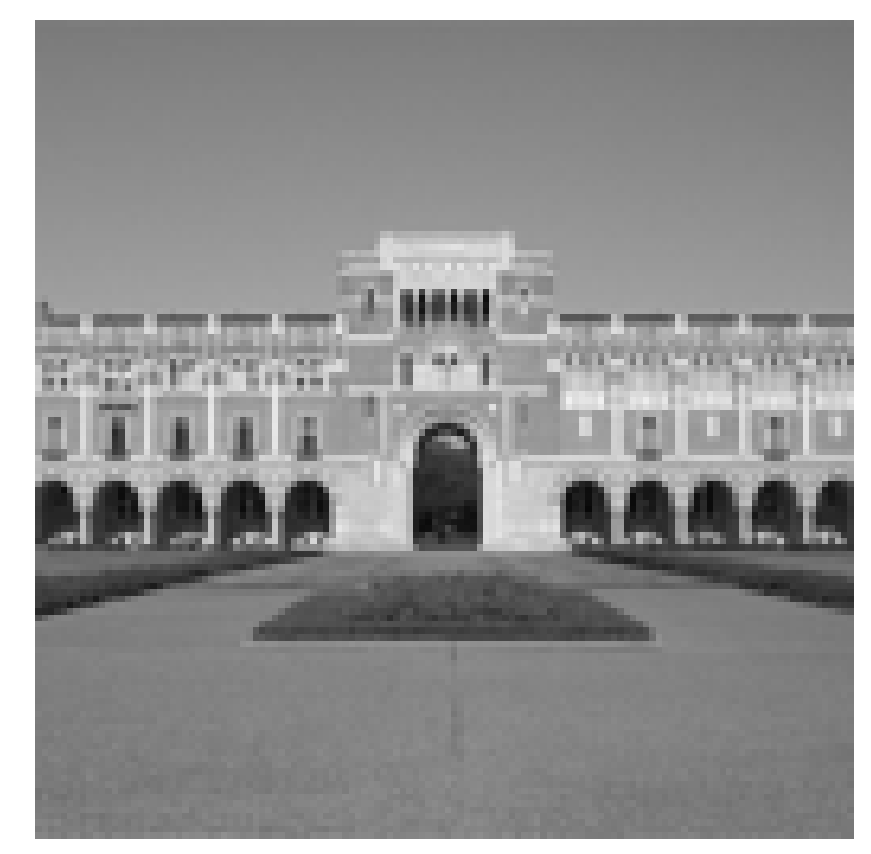
\includegraphics[width=0.24\linewidth]{./fig/lovett_original.pdf} &
		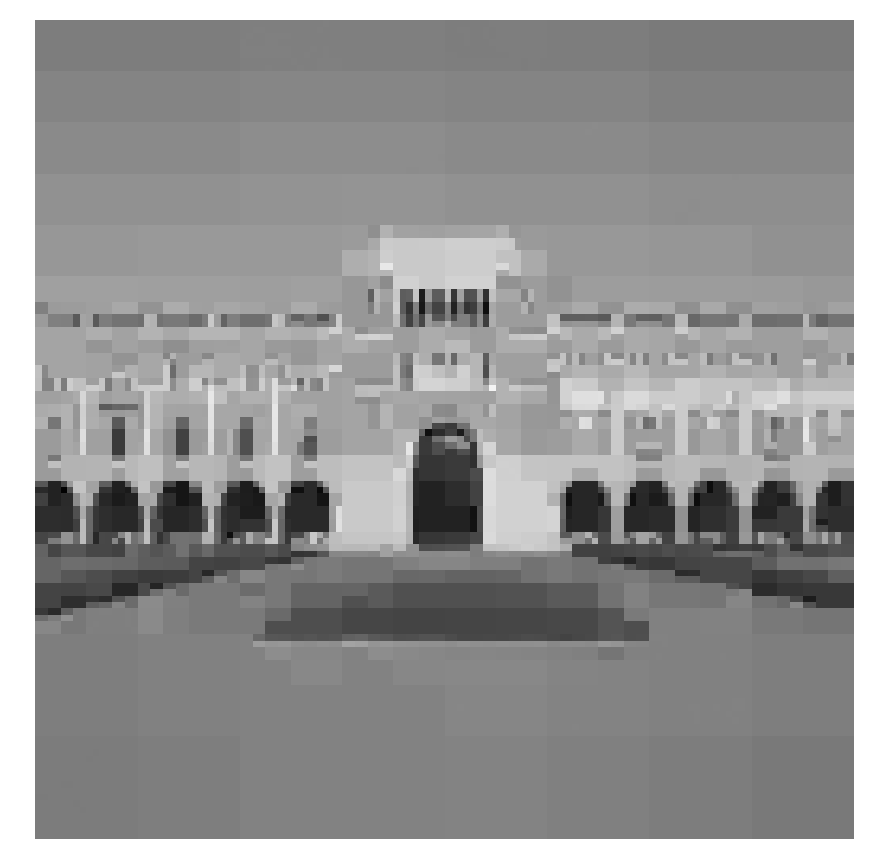
\includegraphics[width=0.24\linewidth]{./fig/lovett_r1.pdf} &
		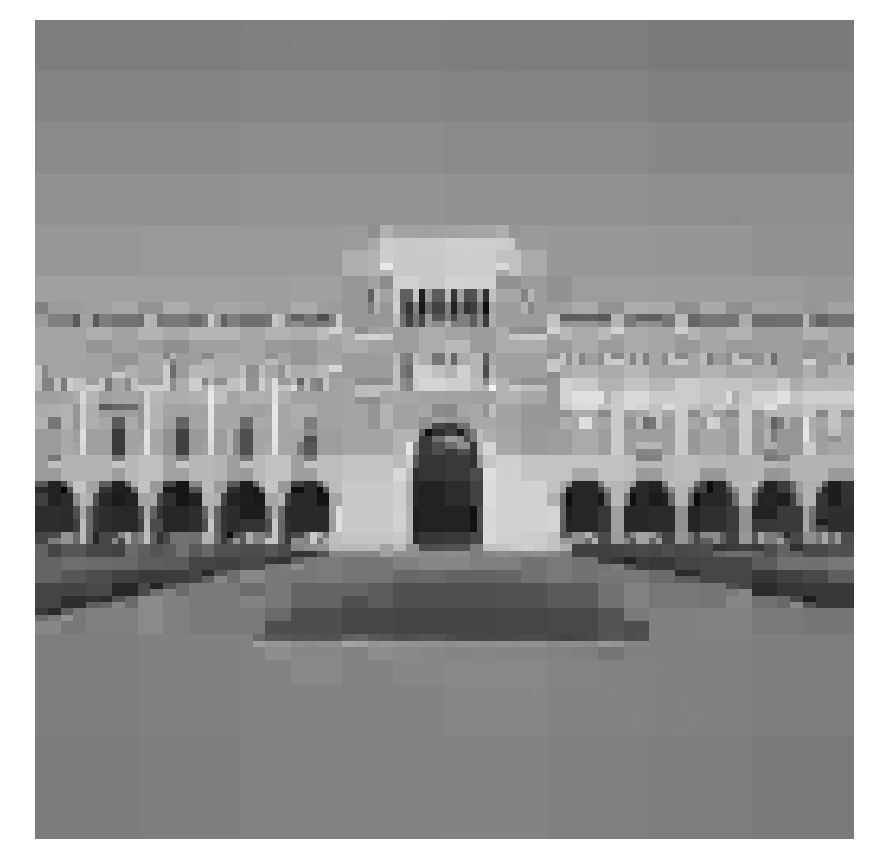
\includegraphics[width=0.24\linewidth]{./fig/lovett_r2.pdf} &
		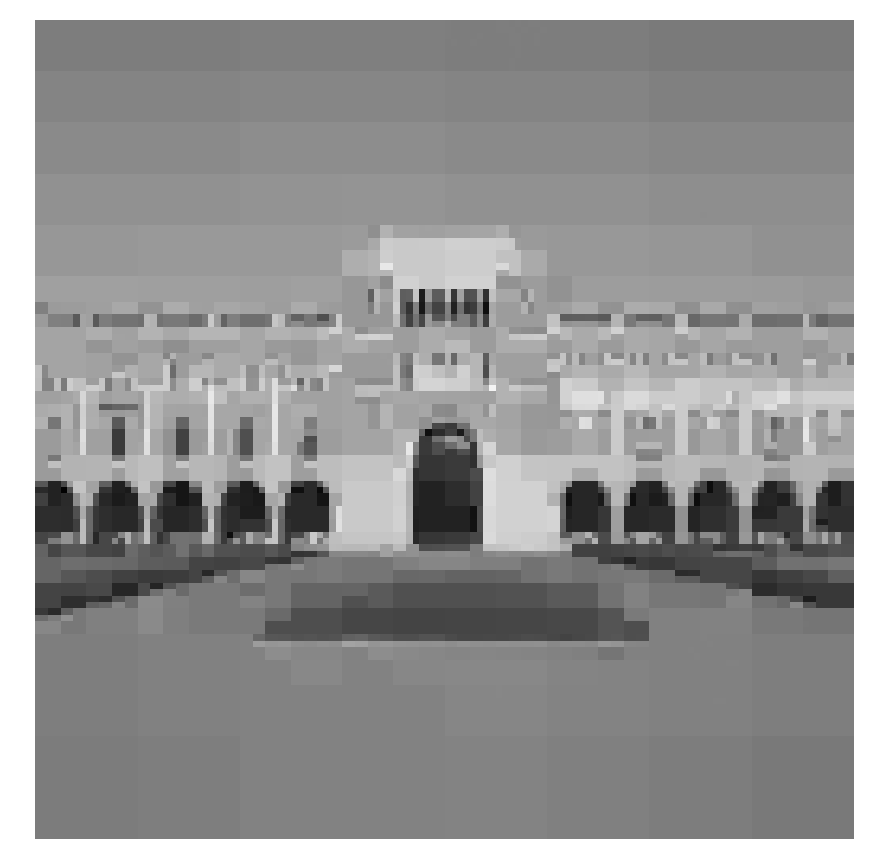
\includegraphics[width=0.24\linewidth]{./fig/lovett_r4.pdf}  \\
		(a) & (b) & (c) & (d)
	\end{tabular}
	\end{center}
	\caption{{(a) Original Lovett Hall image ($n=16,384$); sparse reconstructions ($s=1000$) using $m=8000$ measurements for (b) $R=1$, (c) $R=2$, (d) $R=4$}}
	\label{fig:lovett}
\end{figure*}

%\begin{figure}[h]
%	\begin{center}
%		%\vspace{-0em}
%		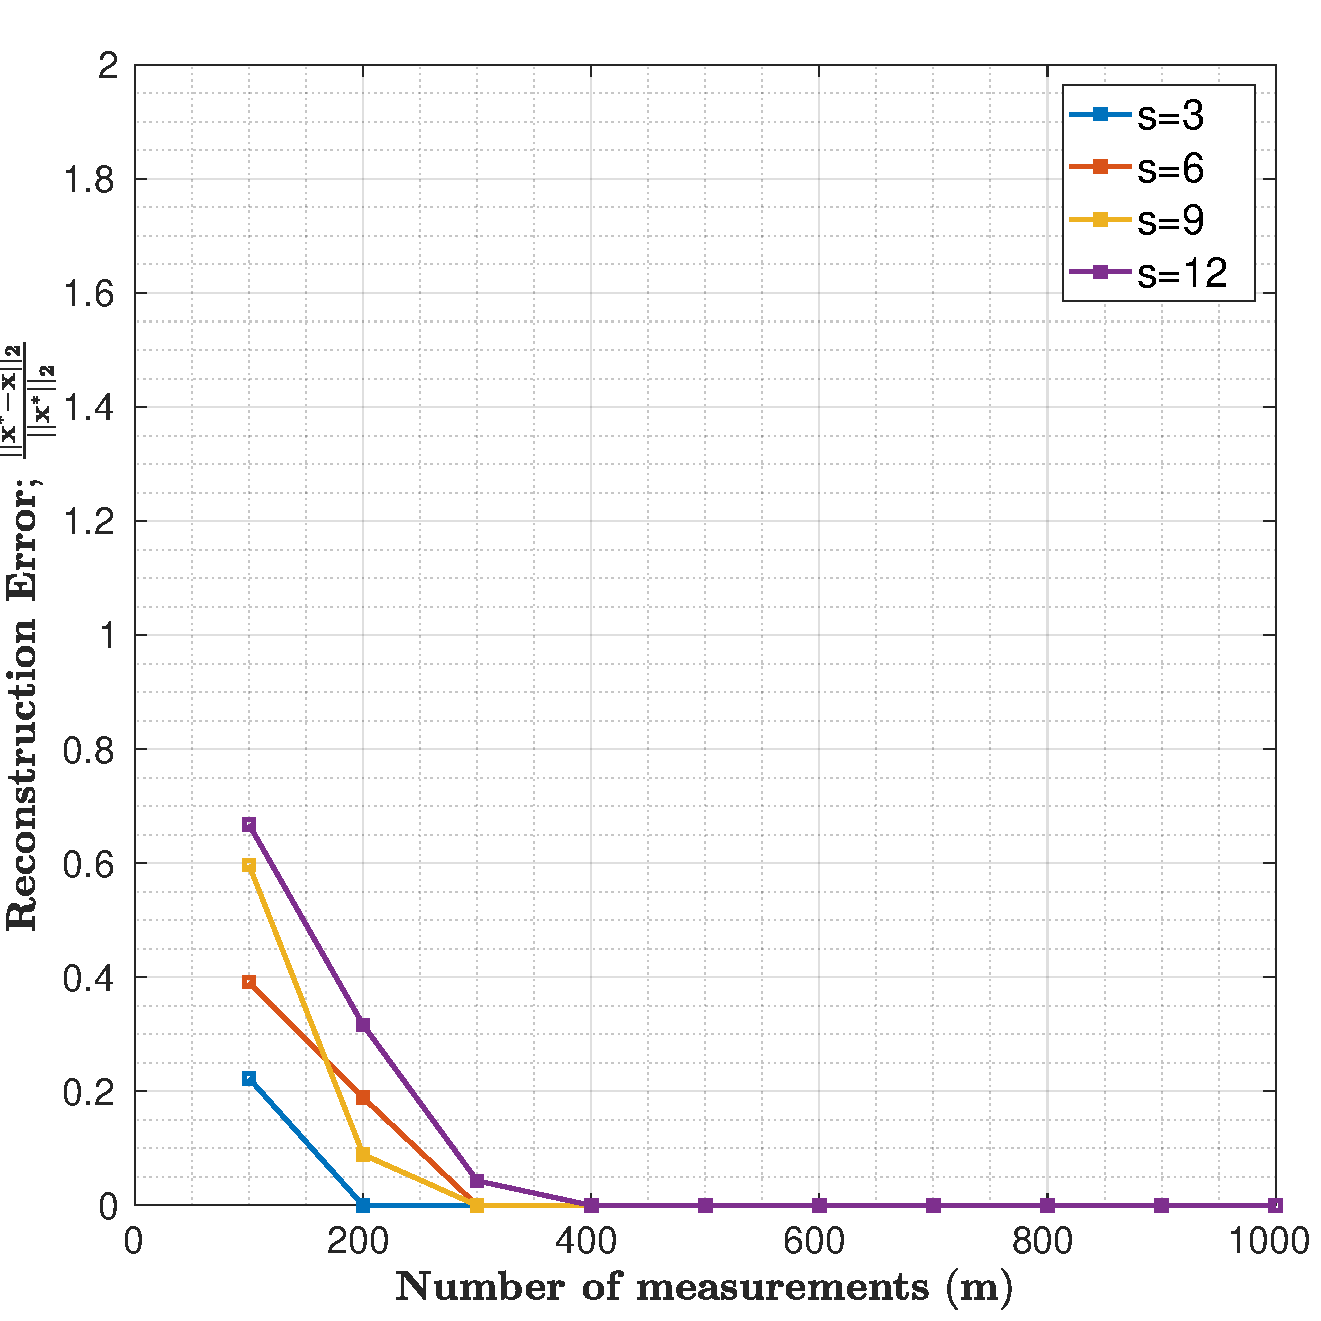
\includegraphics[width=0.9\linewidth]{./fig/rconst_rcm_amp_1_r_1_s_3_12_m_100_1000_justice-pursuit.pdf}
%	\end{center}
%	\caption{{Mean relative reconstruction error vs no. of measurements $(m)$ for MoRAM with $\norm{\mb{x^*}}_2=1,R=1,n=1000$.}}
%	\label{fig:plot-r-1}
%\end{figure}


%\begin{figure}[t]
%	\begin{center}
%		%\vspace{-0em}
%		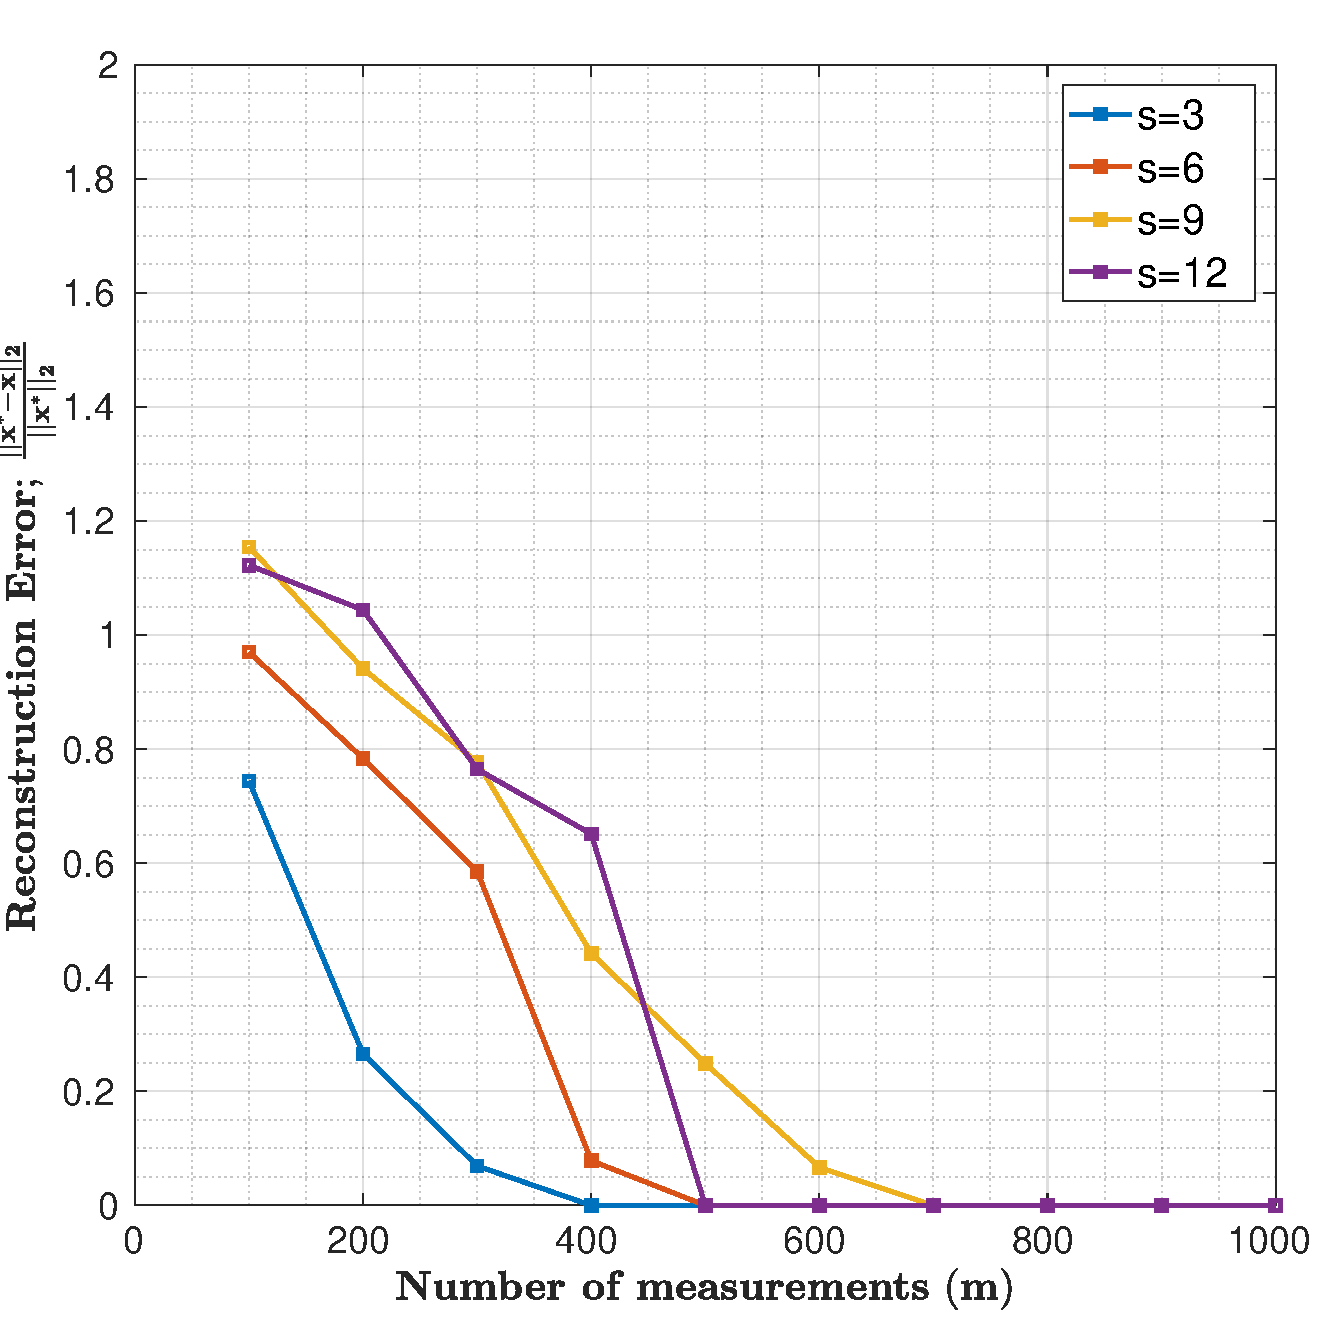
\includegraphics[width=0.9\linewidth]{./fig/rconst_rcm_amp_1_r_2_s_3_12_m_100_1000_justice-pursuit.pdf}
%	\end{center}
%	\caption{{Mean relative reconstruction error vs no. of measurements $(m)$ for MoRAM with $\norm{\mb{x^*}}_2=1,R=2,n=1000$.}}
%	\label{fig:plot-r-2}
%\end{figure}
%
%
%\begin{figure}[t]
%	\begin{center}
%		%\vspace{-0em}
%		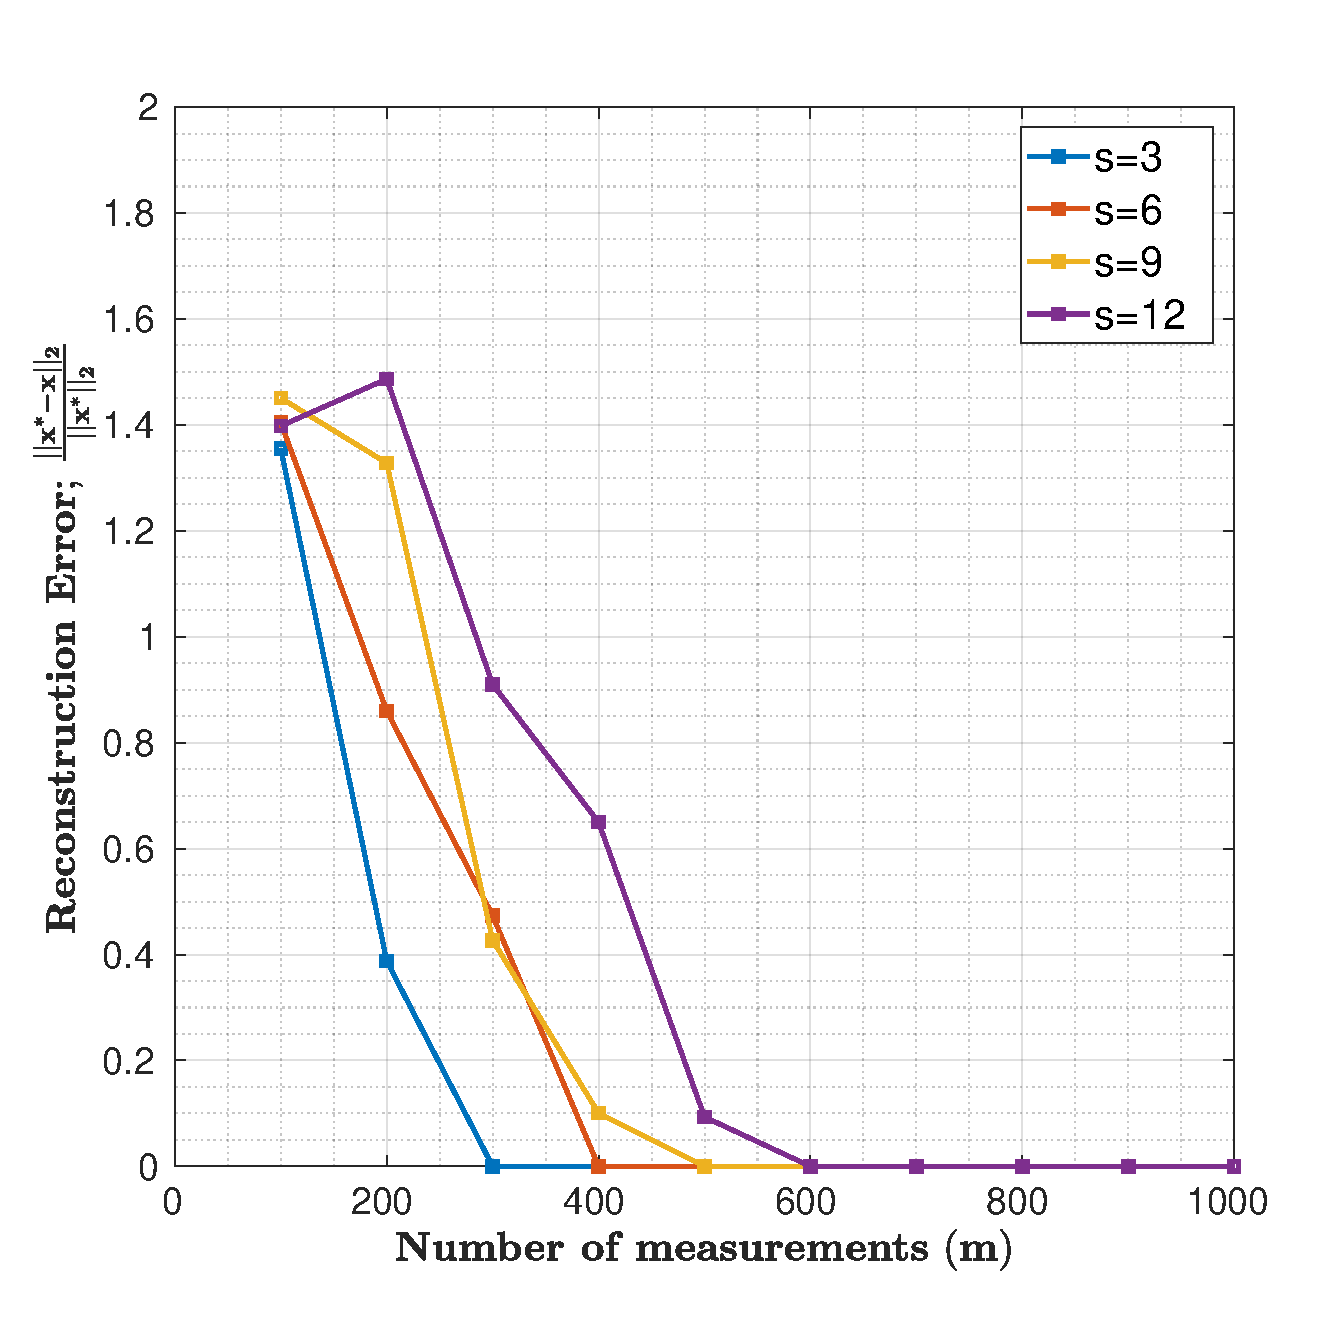
\includegraphics[width=0.9\linewidth]{./fig/rconst_rcm_amp_1_r_4_s_3_12_m_100_1000_justice-pursuit.pdf}
%	\end{center}
%	\caption{{Mean relative reconstruction error vs no. of measurements $(m)$ for MoRAM with $\norm{\mb{x^*}}_2=1,R=4,n=1000$.}}
%	\label{fig:plot-r-4}
%\end{figure}


%\begin{figure}[h]
%	\begin{center}
%		%\vspace{-0em}
%		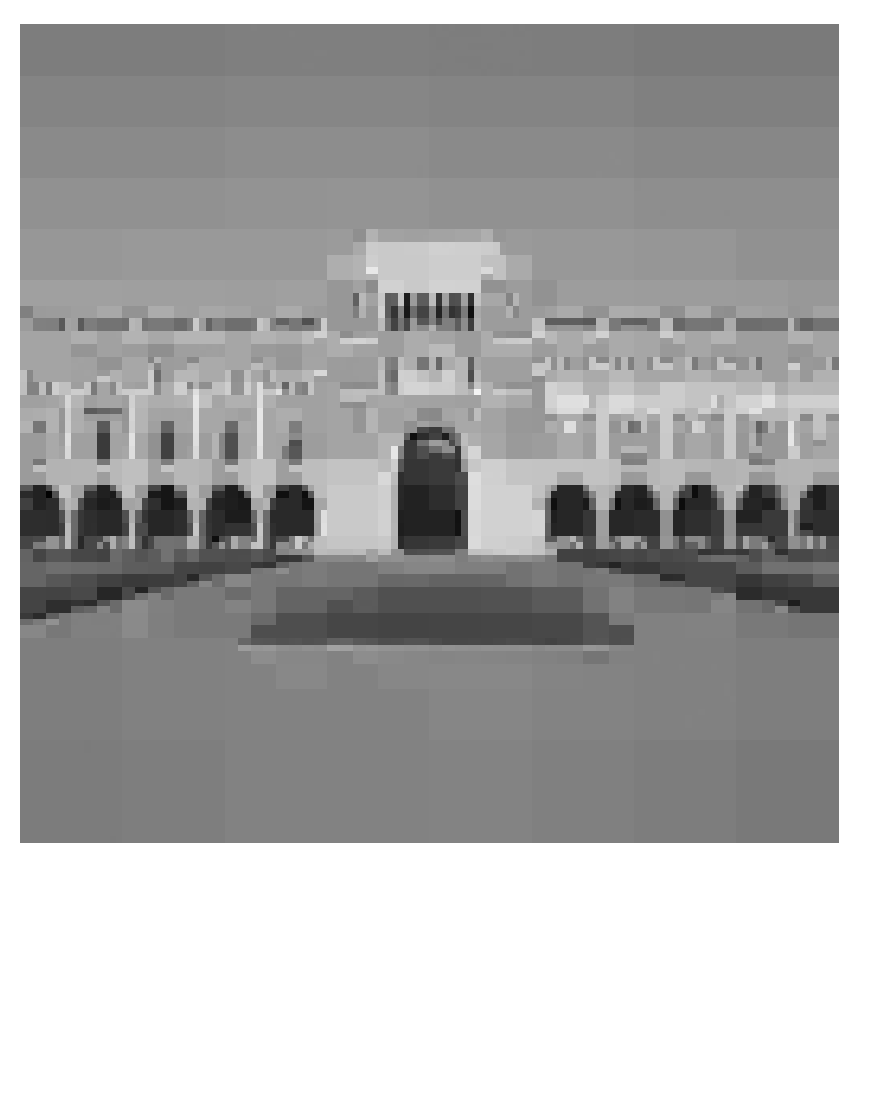
\includegraphics[width=0.9\linewidth]{./fig/reconst_lovett.pdf}
%	\end{center}
%	\caption{{Reconstruction using MoRAM}}
%	\label{fig:lovettreconst}
%\end{figure}
\begin{figure}[!t]
	\centering
	\begin{tikzpicture}
\begin{axis}
[width=0.3\textwidth,
xlabel= Number of samples $m$, 
ylabel= Relative error $\frac{\norm{\mb{x^*-x}}_2}{\norm{\mb{x^*}}_2}$,
grid style = dashed,
grid=both,
legend style=
{
at={(1,1), %for arxiv version
%at={(1.65,0.8),  %for NIPS version
anchor=top},
cells={align=center}, 
%legend columns=-1,
} 
]

\addplot[color=blue,mark=square*] plot coordinates {
	(100, 0.222952795500352)
	(200, 8.25E-05)
	(300, 6.48E-05)
	(400, 6.37E-05)
	(500, 7.91E-05)
 	(600, 6.45E-05)
	(700, 5.51E-05)
	(800, 4.77E-05)
	(900, 6.78E-05)
	(1000, 5.76E-05)
};
\addlegendentry{$s=3$};


\addplot plot coordinates {
(100,	0.391717206388554)
(200,	0.189009904901885)
(300,	8.75E-05)
(400,	6.63E-05)
(500,	7.39E-05)
(600,	6.96E-05)
(700,	5.79E-05)
(800,   6.41E-05)
(900,	8.06E-05)
(1000,	6.78E-05)
};

\addlegendentry{$s=6$};


\addplot[color=green,mark=*] plot coordinates {
(100,0.596874049564358)
(200,0.0893297570309944)
(300,0.0000961819292563893)
(400,0.0000965366166880477)
(500,0.0000950192717929039)
(600,0.0000992956375702069)
(700,0.0000835965044892149)
(800,0.0000675354618845817)
(900,0.0000811820156888768)
(1000,0.000064977150825922)
};
\addlegendentry{$s=9$};

\addplot[color=orange,mark=*] plot coordinates {
(100,0.667881390121055)
(200,0.316701449929789)
(300,0.0432277244535189)
(400,0.000108785027973407)
(500,0.0000962070190416804)
(600,0.0000899199807562489)
(700,0.000102447155819804)
(800,0.0000922462885218879)
(900,0.0000888147784526045)
(1000,0.0000753141220088111)

};
\addlegendentry{$s=12$};



%\legend{CoPRAM\\Block CoPRAM\\ThWF\\SPARTA\\}

\end{axis}
\end{tikzpicture}
	\caption{\sl Mean relative reconstruction error vs no. of measurements $(m)$ for MoRAM with $\norm{\mb{x^*}}_2=1,R=1,n=1000$.} \label{fig:plot-r-1}
\end{figure}

\begin{figure}[!t]
	\centering
	\begin{tikzpicture}
\begin{axis}
[width=0.4\textwidth,
xlabel= Number of samples $m$, 
ylabel= Reconstruction error $\frac{\norm{\mb{x^*-x}}_2}{\norm{\mb{x^*}}_2}$,
grid style = dashed,
grid=both,
legend style=
{
	at={(1,1), %for arxiv version
		%at={(1.65,0.8),  %for NIPS version
		anchor=top},
	cells={align=center}, 
	%legend columns=-1,
} 
]

\addplot[color=blue,mark=square*] plot coordinates {
	(100,0.74427083497336)
	(200,0.26556282505296)
	(300,0.0693282329160152)
	(400,0.0000759947449506268)
	(500,0.0000703837475666469)
	(600,0.0000522047439857151)
	(700,0.0000638145267540324)
	(800,0.000053588062967525)
	(900,0.0000341906002745844)
	(1000,0.0000649790103329161)
	
};
\addlegendentry{$s=3$};


\addplot plot coordinates {
	(100,0.970200248504512)
	(200,0.783733967580109)
	(300,0.585896829880407)
	(400,0.0785807046200051)
	(500,0.0000841836424731131)
	(600,0.0000758879406272977)
	(700,0.0000712248016620914)
	(800,0.0000609478657003822)
	(900,0.0000823001981803784)
	(1000,0.0000652284523240285)
	
};

\addlegendentry{$s=6$};


\addplot[color=green,mark=*] plot coordinates {
	(100,1.15475705568194)
	(200,0.941209335557007)
	(300,0.777520369268922)
	(400,0.442101179084315)
	(500,0.249049460556818)
	(600,0.066874088406845)
	(700,0.0000934401692366995)
	(800,0.0000832753637218933)
	(900,0.0000718321294789104)
	(1000,0.0000674942823198963)
	
};
\addlegendentry{$s=9$};

\addplot[color=orange,mark=*] plot coordinates {
	(100,1.12249994092088)
	(200,1.04403070665004)
	(300,0.76510361311149)
	(400,0.65138560583711)
	(500,0.000087283006450878)
	(600,0.000101093733403955)
	(700,0.0000771972799083333)
	(800,0.0000768498307046639)
	(900,0.0000962856213515402)
	(1000,0.0000790639986588349)
};
\addlegendentry{$s=12$};



%\legend{CoPRAM\\Block CoPRAM\\ThWF\\SPARTA\\}

\end{axis}
\end{tikzpicture}
	\caption{\sl Mean relative reconstruction error vs no. of measurements $(m)$ for MoRAM with $\norm{\mb{x^*}}_2=1,R=2,n=1000$.} \label{fig:plot-r-2}
\end{figure}

\begin{figure}[!t]
	\centering
	\begin{tikzpicture}
\tikzstyle{every node}=[font=\Large]
\begin{axis}
[width=\linewidth,
xlabel= Number of samples $m$, 
ylabel= Relative error $\frac{\norm{\mb{x^*-x}}_2}{\norm{\mb{x^*}}_2}$,
grid style = dashed,
grid=both,
legend style=
{
at={(1,1), %for arxiv version
%at={(1.65,0.8),  %for NIPS version
anchor=top},
cells={align=center}, 
%legend columns=-1,
} 
]

\addplot[color=blue,mark=square*] plot coordinates {
(100,1.35491249236152)
(200,0.387834861360979)
(300,0.0000838932462760031)
(400,0.0000796709195404289)
(500,0.0000699847485553827)
(600,0.0000654248964096406)
(700,0.0000556622044076941)
(800,0.0000577754338669424)
(900,0.0000476093461140991)
(1000,0.000050430624642886)

};
\addlegendentry{$s=3$};


\addplot plot coordinates {
(100,1.4044226284938)
(200,0.860030446367654)
(300,0.473492899335313)
(400,0.0000833934372627376)
(500,0.0000824008767554939)
(600,0.0000637716674864768)
(700,0.0000644672859553126)
(800,0.0000649831938234799)
(900,0.0000692018122982395)
(1000,0.0000633648746645319)

};

\addlegendentry{$s=6$};


\addplot[color=green,mark=*] plot coordinates {
(100,1.45063072923552)
(200,1.32791017206988)
(300,0.426899433442911)
(400,0.100521404653474)
(500,0.0000847861906819546)
(600,0.0000874052339854557)
(700,0.0000975048393826316)
(800,0.000072296472052776)
(900,0.0000706944130642887)
(1000,0.0000730819848601016)

};
\addlegendentry{$s=9$};

\addplot[color=orange,mark=*] plot coordinates {
(100,1.39786595436235)
(200,1.48655013005159)
(300,0.909955665520478)
(400,0.649802110302209)
(500,0.0932660496014009)
(600,0.0000913091790977068)
(700,0.000104507094662964)
(800,0.0000965628384101342)
(900,0.0000934605996504098)
(1000,0.0000841210242777489)	
};
\addlegendentry{$s=12$};



%\legend{CoPRAM\\Block CoPRAM\\ThWF\\SPARTA\\}

\end{axis}
\end{tikzpicture}
	\caption{\sl Mean relative reconstruction error vs no. of measurements $(m)$ for MoRAM with $\norm{\mb{x^*}}_2=1,R=4,n=1000$.} \label{fig:plot-r-4}
\end{figure}


\section{Appendix}
\label{sec:append}
%\clearpage
%\input{../common/ack}
\bibliographystyle{plain}
\bibliography{./vsbib}
%\input{../common/appendix_a}
%\input{../common/appendix_b}

\end{document}